\chapter{Методы генерации двойных оптических гребенок и солитонов в кристаллических микрорезонаторах} \label{chapt4}

\section{Генерация двух солитонных оптических гребенок в двух резонаторах на одном цилиндре}

Для одновременной генерации нескольких солитонных оптических гребенок \cite{Pavlov2017} с практически идентичными частотами повторения были разработаны структуры с несколькими резонаторами одинаковой формы, выточенными на одном кристаллическом цилиндре из $MgF_2$ (рис. \ref{ris:image1}). Стэк резонаторов имеет пять одинаковых выступов с радиусом кривизны 35 мкм и радиусом цилиндра 2.84 мм (ОСД около 12.1 ГГц). Расстояние между соседними по высоте резонаторами 140 мкм. Такой стэк микрорезонаторов был изготовлен острым резцом с радиусом кривизны 4 мкм на станке алмазного точения.

\begin{figure}[!htb]
\begin{minipage}{1\linewidth}
\center{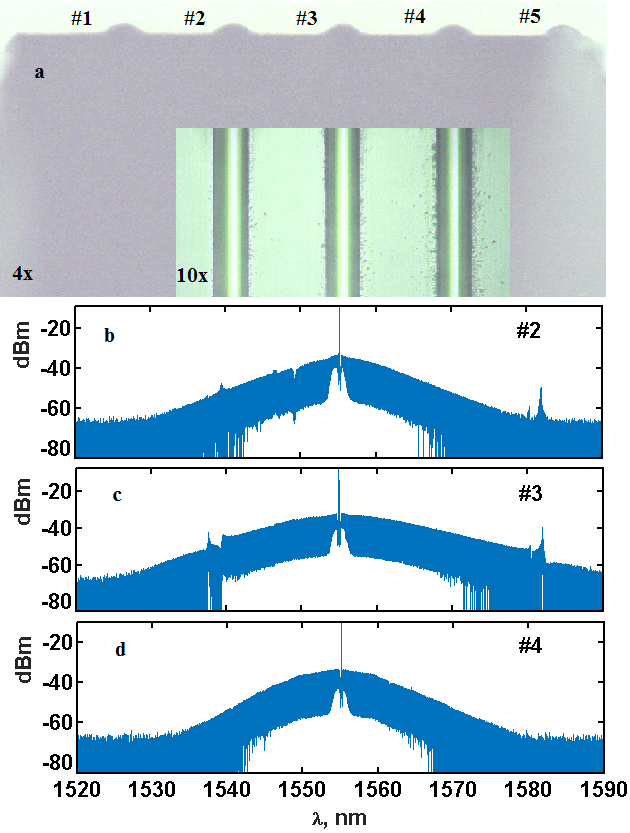
\includegraphics[width=0.5\linewidth]{dual_cavity}}
\end{minipage}
\caption{(a): Фото стэка резонаторов на одном кристаллическом цилиндре с диаметром 5.68 мм (зазор между соседними выступами около 140 мкм, радиус кривизны поверхности выступа 35 мкм). Вставка показывает 3 отполированных выступа (номера 2 -- 4), в которых наблюдались солитоны; (b-d): оптический спектр солитонов, генерируемых в 3 различных резонаторах. Солитонные керровские частотные гребенки имеют ширину $30 - 65$ нм с расстоянием 12.1 ГГц.}
\label{ris:image1}
\end{figure}

Добротность сразу после алмазного точения без полировки составила порядка 10$^6$. Добротность больше $10^9$ была достигнута асимптотической последовательной полировкой алмазными суспензиями. В результате финальной полировки разница в ОСД между несколькими выступами была не более 10 МГц, что соответствует разнице в радиусах резонаторов в $0.5 - 1$ мкм при условии возбуждении одного семейства мод в обоих резонаторах.

\begin{figure}[!htb]
\begin{minipage}{1\linewidth}
\center{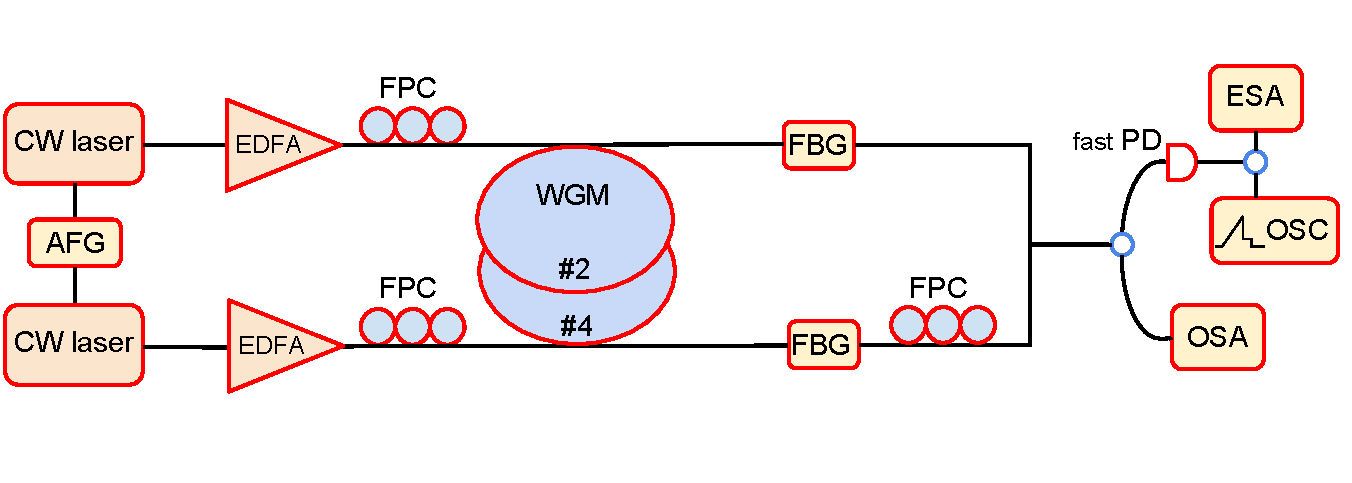
\includegraphics[width=0.75\linewidth]{dual_setup}}
\end{minipage}
\caption{Экспериментальная установка по генерации солитонных двойных гребенок из выступов номер 2 и 4. Лазер: узкополосный перестраиваемый волоконный лазер непрерывной мощности; EDFA: эрбиевый волоконный усилитель; Ген: генератор сигналов произвольной формы; ВКП:  волоконный контроллер поляризации; Ф: оптический фильтр - волоконная Брэгговская решетка; ФД: фотодетектор; ЭСА: анализатор спектра электрических сигналов; ОСА: оптический анализатор спектра; ОСЦ: осциллограф.}
\label{ris:image2}
\end{figure}

Схема экспериментальной установке дала на рис. \ref{ris:image2}.  Два независимых (не связанных по фазе) узкополосных волоконных лазера непрерывной мощности ($\lambda \sim 1554$~нм) были усилены в эрбиевом волоконном усилителе до 150 мВт и связаны с резонаторами через 2 растянутых волокна. Каждое волокно подносилось для связи к отдельному выступу микрорезонатора (номер 2 и 4) с противоположных сторон цилиндра, в которых возбуждаются солитоны с различными ОСД. Генератор сигналов произвольной формы использовался для контроля процесса возбуждения солитонов, с него подавался одиночный пилообразный импульс для настройки частоты лазера. Контроллеры поляризации использовались для оптимизации связи с модой резонатора. Фильтр на волоконной Брэгговской решетке использовался для подавления мощной накачки на выходе после микрорезонаторов.

Частоты повторения солитонов наблюдались на быстром фотодетекторе (ширина полосы 26 ГГц) и широкополосном анализаторе спектра электрических сигналов. Для  оптического спектра использовался оптический спектроанализатор с решеткой. На осциллографе наблюдались характерные для солитонов ступеньки в генерируемом и проходящем свете.

\begin{figure}[!htb]
\begin{minipage}{1\linewidth}
	\center{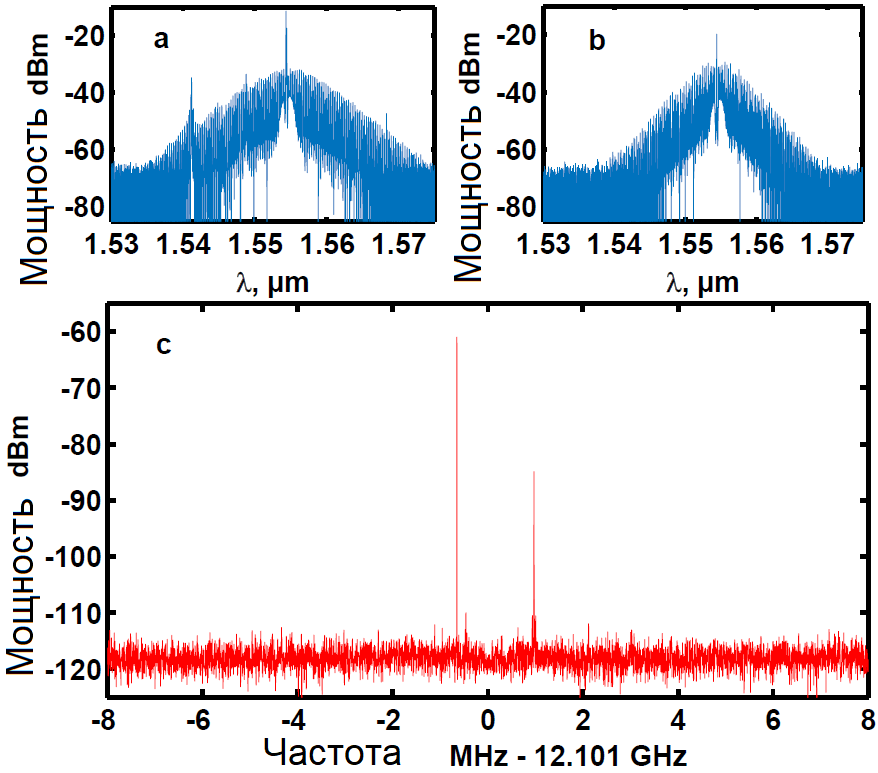
\includegraphics[width=0.5\linewidth]{dual_comb_osa}}
\end{minipage}
\caption{(a-b): Оптические спектры мультисолитонных режимов, возбужденные в двух различных резонаторах; (c): сигнал биений на частотах повторений от двух солитонов в разных резонаторах, разница в частотах $1.62$ МГц.}
\label{ris:image3}
\end{figure}

Солитоны были получены последовательно в 3 из 5 резонаторах на 1 цилиндре (Рис. \ref{ris:image1}). Ширина спектра оптических солитонов (Рис.\ref{ris:image1}(b) -- рис.\ref{ris:image1}(d)) составила 30-65 нм около 1554 нм. Разница между частотами лазеров накачки была $8.9-30$ пм. Две солитонные оптические гребенки с разницей в частотах повторений $\Delta\mbox{FSR} = \mbox{FSR}_1 - \mbox{FSR}_2 = 1.62$~МГц были одновременно возбуждены в двух микровыступах на 1 кристаллическом цилиндре и далее совмещены на волоконном делителе. Для настройки на солитоны использовался метод, предложенный в \cite{Herr2014}. Пилообразный однократный сигнал подавался одновременно на оба лазера, начальная точка перестройки выбиралась путем совмещения солитонных ступенек, т.ч. финальная отстройка лазеров попадала в область существования солитонов в обоих резонаторов. Область существования солитонов составляла не более 8 МГц по отстройке, поэтому необходимо было так подобрать мощности лазеров, чтобы в обоих резонаторах эти области были приблизительно одинаковые. Совмещение достигалось благодаря плавной подстройке частоты каждого лазера.

Оптические спектры мультисолитонных гребенок в обоих резонаторах даны на рис.~\ref{ris:image3}(a) -- ~\ref{ris:image3}(b), самая узкая гребенка на рис.~\ref{ris:image3}(b) содержит более 300 значимых линий, разделенных по $12.1$ ГГц и покрывает 35 нм около центральной частоты $\lambda = 1554$~нм. Разница в частотах лазеров накачки была $1.07$~ГГц. Результирующий сигнал биений на фотодетекторе от двух оптических гребенок отображает двойную оптическую гребенку в радиодиапазон (Рис. \ref{ris:image4}, \ref{ris:dual_comb_individual_lines}), имеет общую ширину 300 МГц с центром на 1.07 ГГц и содержит около 150 линий, разделенных на $1.62$ МГц, и имеет огибающую, совпадающую с оптическими профилями двух солитонов. Время жизни двойной оптической гребенки было не более 20 секунд, т.к. не была выполнена никакая стабилизация частот лазеров накачки и температуры цилиндра. На рис. \ref{ris:dual_comb_individual_lines} показана ширина индивидуальных линий (около 200 кГц) в СВЧ диапазоне в другой реализации эксперимента, когда солитоны возбуждались на других семействах мод в двух различных резонаторах.

\begin{figure}[!htb]
\begin{minipage}{1\linewidth}
\center{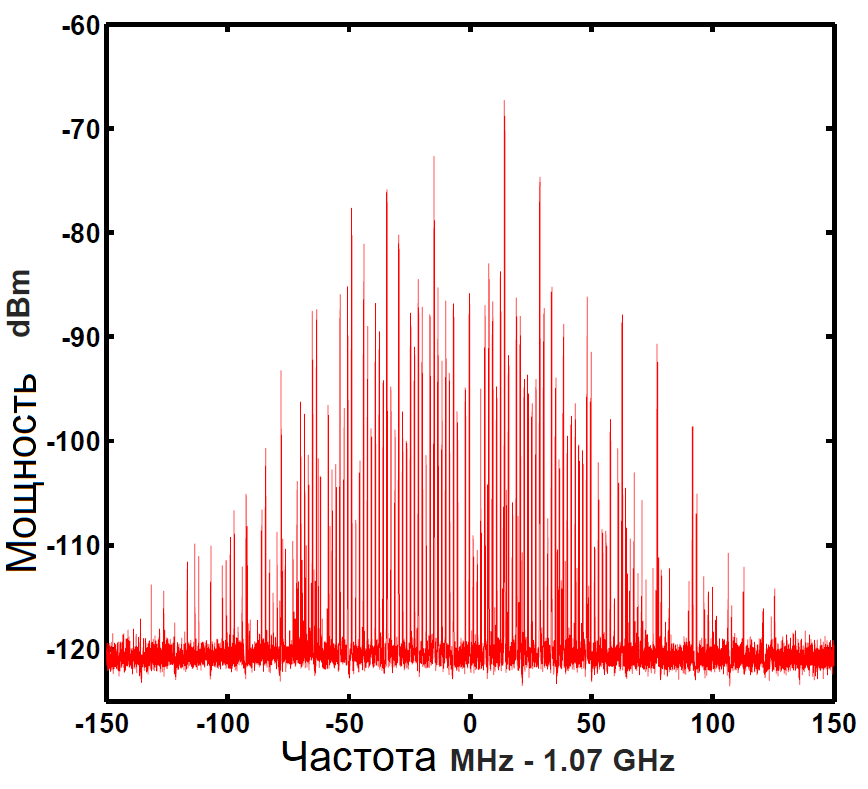
\includegraphics[width=0.5\linewidth]{dual_comb_esa}}
\end{minipage}
\caption{СВЧ спектр результата биений двух солитонных оптических частотных гребенок. СВЧ спектр покрывает 300 МГц с центральной частотой 1.07 ГГц, состоит из 160 линий с расстоянием между ними 1.62 МГц}
\label{ris:image4}
\end{figure}

\begin{figure}[!htb]
\begin{minipage}{1\linewidth}
	\center{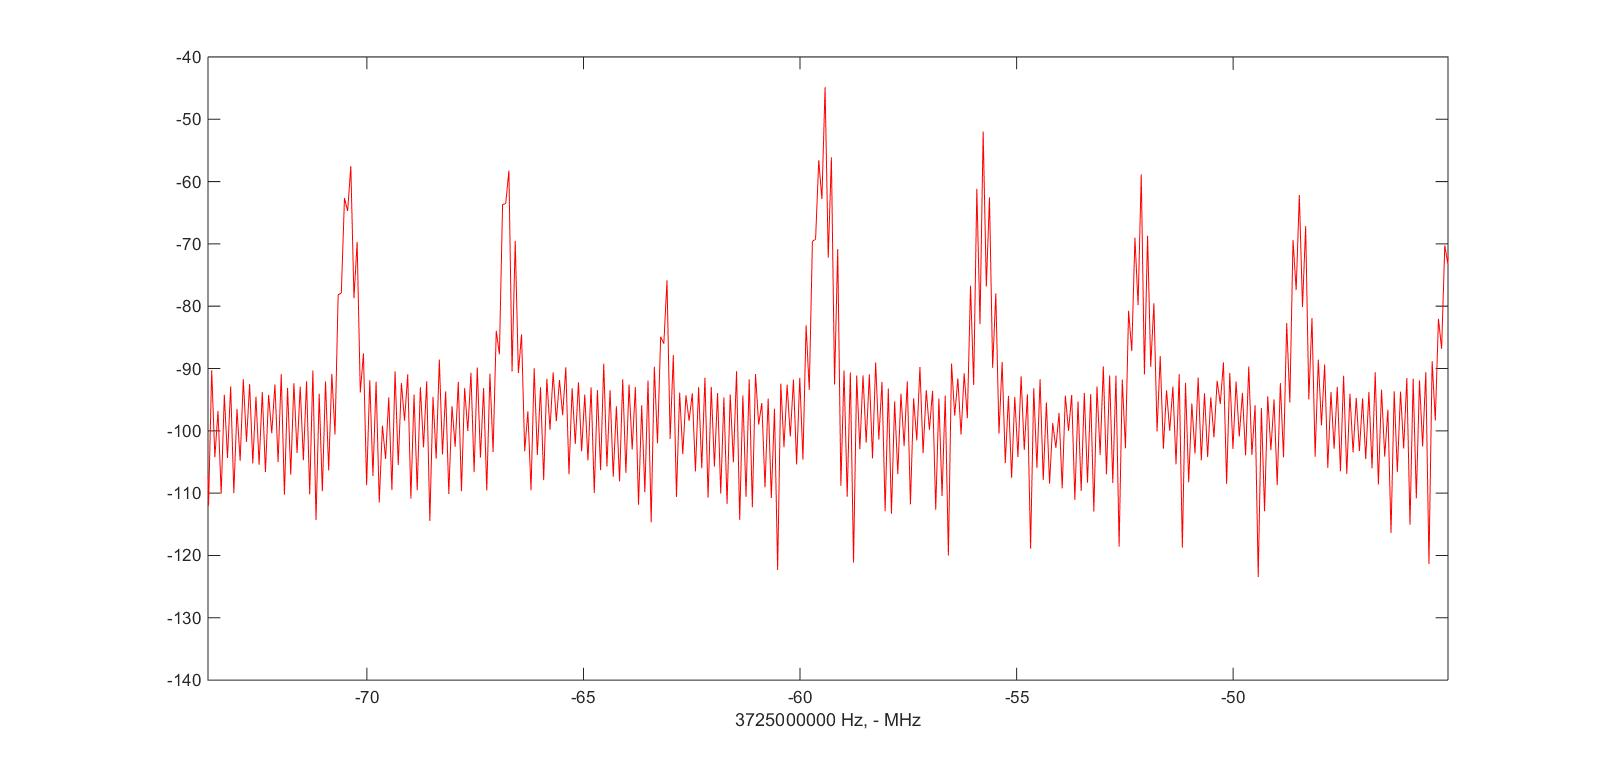
\includegraphics[width=0.5\linewidth]{dual_comb_individual_lines}}
\end{minipage}
\caption{Индивидуальные линии радиочастотной гребенки, ширина каждой порядка 1 МГц, что указывает на невысокую взаимную когерентность двух оптических гребенок из-за использования двух независимых лазеров, не привязанных по фазе.}
\label{ris:dual_comb_individual_lines}
\end{figure}

Короткое время жизни двойной гребенки обусловлено тепловым сдвигом резонансных частот. Наблюдалось, что возбуждение солитона в одном резонаторе приводило к сдвигу резонанса в другом резонаторе, т.ч. эффективная отстройка оказывалась вне области существования солитона. В результате, как правило, наблюдалось одновременное возбуждение солитона в одном резонаторе и шумной гребенки (модуляционной неустойчивости) в другом резонаторе. Типичный экспериментально наблюдаемый тепловой сдвиг при возбуждении солитона в соседнем резонаторе составляет 30-50 МГц. Несмотря на большое расстояние между резонаторами в 140 мкм, через элемент связи одного резонатора можно было наблюдать моды другого резонатора и даже гребенку в другом резонаторе (по уровню -30 дБ), что говорит о большом рассеянии внутри цилиндра и недостаточной локализации поля в выступе с радиусом 35 мкм и высотой около 10 мкм. Для уменьшения теплового влияния можно разнести резонаторы на одном цилиндре более, чем на 3 мм, использовать меньшую мощность накачки (порядка 50 мВт, что требует более высокой добротности резонаторов) или создать активную систему термостабилизации.

\section{Генерация солитонных оптических гребенок в одном резонаторе на разных семействах мод в одном направлении}

Генерация двойных оптических частотных гребенок в отдельных независимых резонаторах с помощью двух независимых лазеров, не привязанных друг к другу по фазе, имеет ряд минусов: необходимость точить и полировать два резонатора с высокой добротностью и разницей в диаметрах на уровне единиц микрон, также усложняется экспериментальная схема: удваивается количество оптических элементов в экспериментальной установке, требуются дополнительные волоконные изоляторы, волоконные контроллеры поляризации и волоконные оптические делители. Необходимо стабилизировать температуру обоих резонаторов с одинаковой точностью. Даже при реализации всего вышеперечисленного результирующий сигнал двойной гребенки в СВЧ диапазоне имеет мгновенную ширину индивидуальной линии порядка 500 кГц и нестабильность частоты порядка 20 МГц на временах 5 с из-за нестабильности частот лазеров накачки и различными тепловыми флуктуациями двух микрорезонаторов.

Все изготовленные мною в лаборатории кристаллические резонаторы были многомодовыми. Общее количество мод можно снизить, увеличивая отношения диаметра диска к радиусу кривизны боковой грани, или изготавливая микровыступы в форме трапеции острым резцом. Наименьшее количество мод наблюдалось в резонаторе диаметром 5.6 мм и радиусом кривизны боковой грани 35 мкм и в резонаторе 7.5 мм диаметром и с 80 мкм радиусом кривизны боковой грани. При этом при стандартной технике полировки наблюдалось несколько семейств мод с добротностью не менее $10^9$ на 1550 нм.

Пример сканирования широко перестраиваемым лазером большой мощности ОСД резонатора из $MgF_2$ дан на рис. \ref{Scan_SolitonSpot}, видно возбуждение гребенок на большом количестве семейств мод, при этом характерные солитонные ступеньки в генерируемом свете видны на меньшем числе мод, они помечены черным и даны в увеличенном масштабе. Используемый резонатор имел радиус  2.75 мм и радиус кривизны микровыступа около 80 мкм (Рис. \ref{Figure1_V1_c} (a)). Не менее двух мод, поддерживающих генерацию солитонов, были наблюдены и в других резонаторах с ОСД 9.9,14.1,17.6,25.9 ГГц. Все эти резонаторы имели радиус кривизны боковой грани больше 100 мкм.

\begin{figure}[!htb]
\begin{minipage}{1\linewidth}
\center{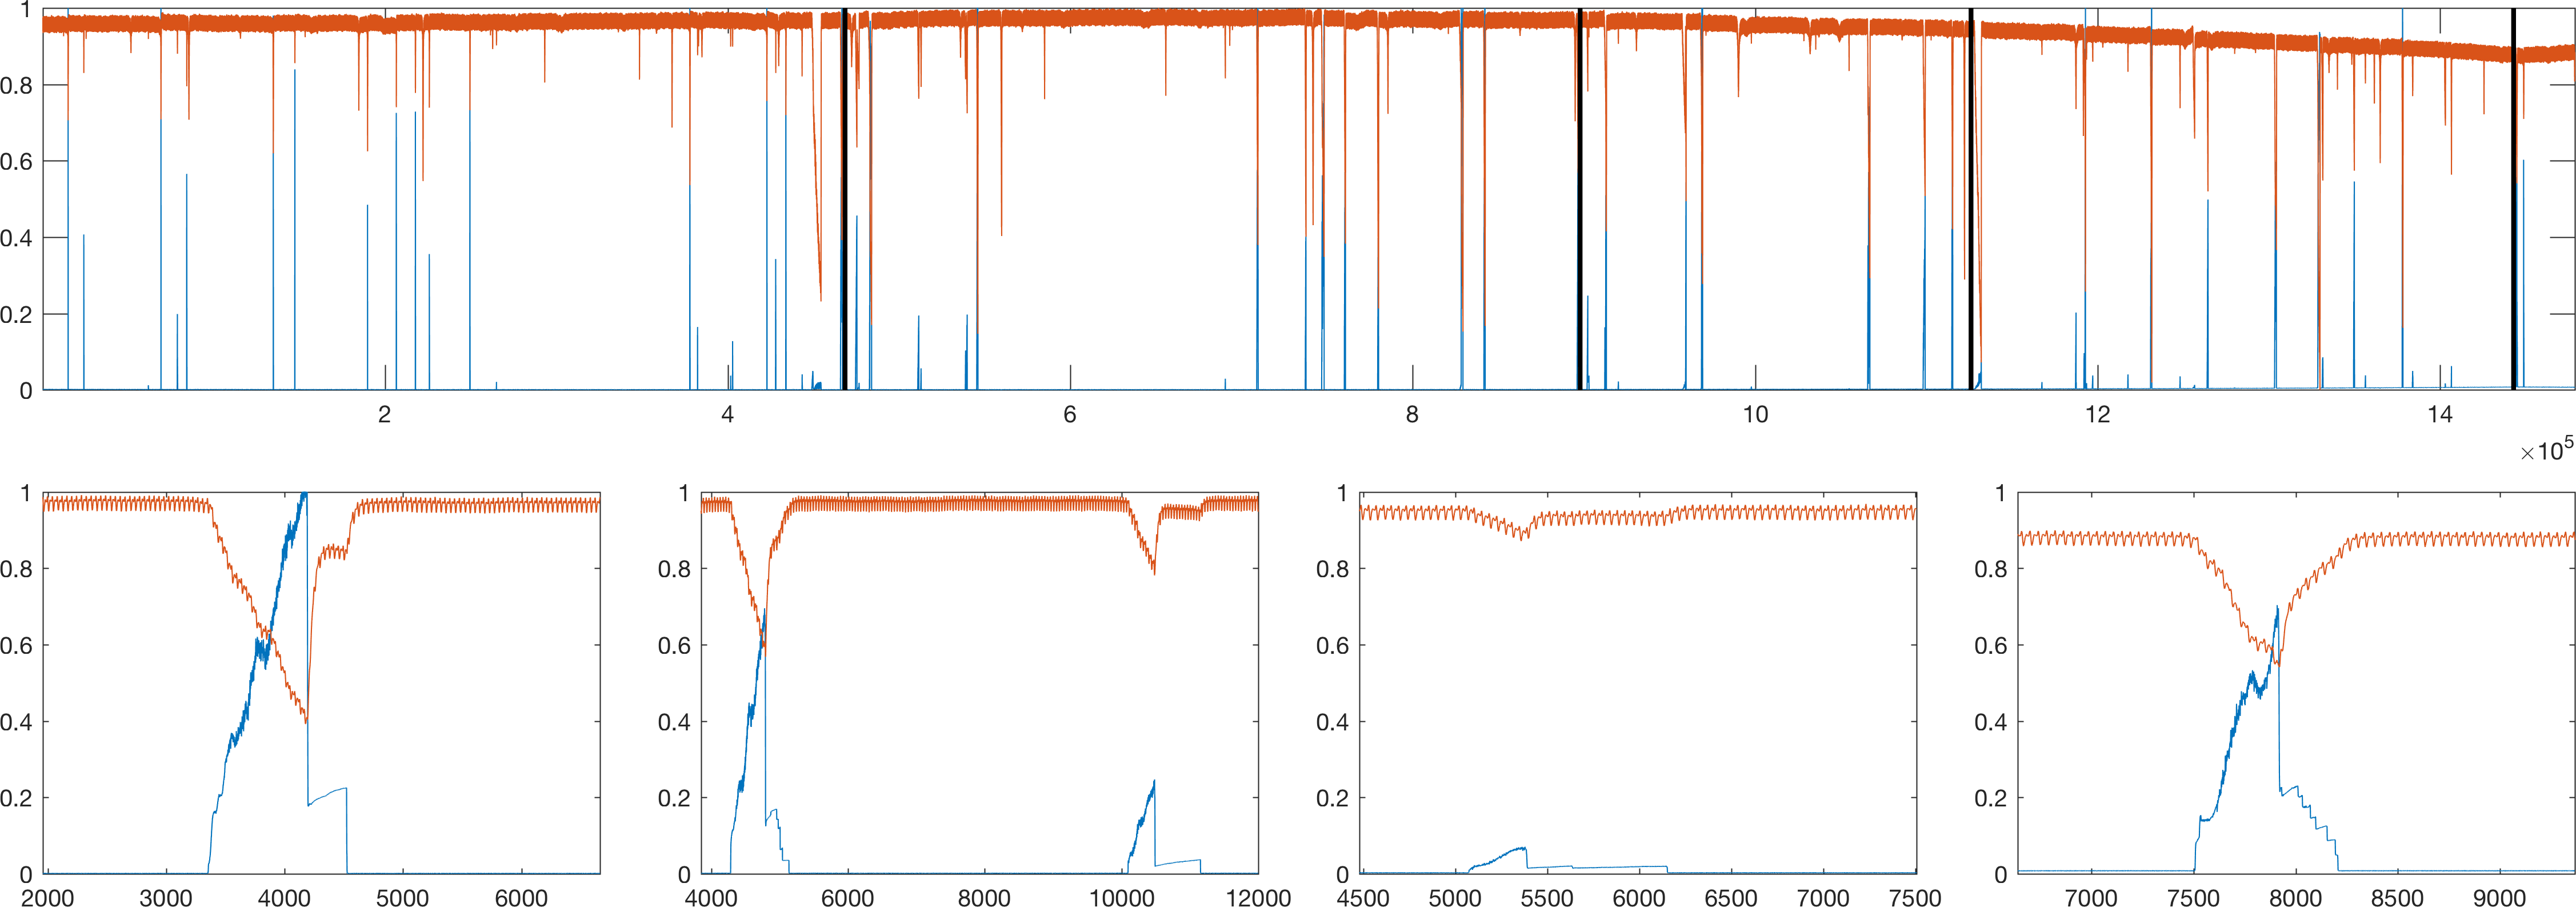
\includegraphics[width=1\linewidth]{Scan_SolitonSpot}}
\end{minipage}
\caption{Сканирование лазером большой мощности 1 ОСД резонатора из $MgF_2$. Сверху красным даны сигналы пропускания системы, синим - генерируемый свет (сигнал пропускания за вычетом отфильтрованного мощного сигнала накачки). Наблюдается большое количество оптических гребенок, генерируемых на разных семействах мод. Черным выделены несколько примеров мод с характерным для генерации солитонов ступеньками в сигнале генерируемого света (даны в увеличенном масштабе в нижнем ряду)}
\label{Scan_SolitonSpot}
\end{figure}

Групповая дисперсия материала $MgF_2$ является аномальной в телекоммуникационном С-диапазоне ($\beta_2=-9$ фс$^2$мм$^{-1}$), и любая геометрия выступа оставляет дисперсию в аномальном диапазоне, что позволяет генерировать светлые солитоны.

Экспериментально в схеме с генерацией солитонов, распространяющихся в одном направлении (Рис. \ref{Figure1_V1_c}), использовался лазер (ECDL на длине волны 1554 нм) и IQ электрооптический модулятор в режиме генерации одной боковой линии. Мощности линии лазера и боковой линии амплитудной модуляции выравнивались, а разность частоты контролировалась с помощью стабильного СВЧ генератора. Для накачки использовались 2 моды из разных семейств с разницей собственных частот около 4 ГГц. Для настройки на солитонный режим использовалась описанная в предыдущих пунктах техника сканирования частоты лазера, но перед этим, подбирая частоту модуляции на IQ модулятор, выравнивались солитонные ступеньки по правому краю (Рис. \ref{Figure2}), по максимальной отстройке области существования солитонов. После этого подавалась однократное пилообразное напряжение на пьезоэлемент лазера для быстрой настройки частоты лазера на нужную отстройку. В половине попыток удавалось достичь генерации солитонного режима в обоих семействах мод. Однако для достижения односолитонного режима требовалось либо оптимизировать связь с модами через микропозиционирование волокна, либо выполнять большее число попыток. Лишь в 1 из 10 случаев генерировались одновременно 2 односолитонных режима. Однако стоит заметить, что при наличии одного возбужденного солитона или просто мощности дополнительного лазера накачки в модах резонатора, достижение солитонного режима во второй моде упрощается и его стабильность повышается за счет улучшения температурной динамики. После достижения солитонного режима включалась схема привязки частоты лазера методом PDH на заданной отстройке, для этого использовался дополнительный фазовый модулятор перед IQ модулятором. Для улучшения шумовых характеристик оптических гребенок была выполнена стабилизацию температуры с помощью элемента Пельтье под латунной подставкой резонатора. Термистор был закреплен достаточно далеко от резонатора и вносил задержку при температурной стабилизации. Температура резонатора стабилизировалось с точностью до 10 мК. Режим двойной гребенки мог существовать несколько часов при отсутствии сильных акустических вибраций.

На рис. \ref{Co_Scheme_results} показаны оптические спектры одновременно двух солитонов на разных семействах мод с разницей по частоте накачки $f_m=4.28$ ГГц. Разница в частотах повторения солитонов составила $\Delta f_{rep}=655$ кГц (около $f_{rep}=12.4$ ГГц), что соответствует фактору сжатия \cite{Coddington2016} $m=f_{rep}/\Delta f_{rep}=1.8\times10^4$, что полезно для увеличения скорости сбора данных электроникой для покрываемого гребенкой небольшого оптического диапазона. Ширина индивидуальных линий результирующей СВЧ гребенки менее 100 Гц и не разрешается прибором (при разрешении спектроанализатора в 100 Гц), хотя вся система не стабилизирована (частота повторения солитонов и лазер накачки не привязаны ни к каким эталонам). Для сравнения был проведен эксперимент по накачке одним лазером и линией амплитудного модулятора двух различных независимых резонаторов (на разных подставках) с близкими ОСД. Генерация двойной гребенки также возможна, однако одновременная настройка на солитонный режим сложнее и тепловая стабильность существенно хуже, т.ч. взаимная когерентность оптических линий, эквивалентная ширине индивидуальной линии СВЧ гребенки, хуже 1 кГц.

Вернемся к эксперименту в одном резонаторе: благодаря высокой частоте $f_m$ и небольшой разнице в частотах повторения, отображение оптического спектра на СВЧ спектр взаимно однозначно, 200 МГц радио спектра отображаются на 3 ТГц оптического диапазона без каких-либо наложений на частоту $f_{rep}-f_m$. В экспериментах с другими парами мод из различных семейств, удавалось найти солитонные резонансы с разницей собственных частот порядка $f_m=100$ МГц, т.ч. потенциально можно обойтись без высокочастотных генераторов, детекторов, анализаторов спектра и осциллографов.

Важно отметить, что хотя солитоны распространяются в различных пространственных модах, они могут эффективно взаимодействовать через четырехволновое взаимодействие, и могут быть модулированными на частоте $\Delta f_{rep}$. Дополнительные оптические линии около каждой линии гребенки будут при биениях с соседними линиями гребенки давать биения на точно такой же частоте, что и биения основных линий гребенки, приводя к не взаимно однозначному отображению в СВЧ область. Условие сохранения углового момента не выполняется при распространении солитонов в противоположных направлениях, но выполняется при распространении в одном направлении для мод с условием $\mu+\eta=\mu^\prime+\eta^\prime$, где $\mu,\eta$ азимутальные числа относительно моды накачки. Например, взаимодействие мод с номерами $\mu+\eta=(\mu-2)+(\eta-2)$ приведет к возникновению оптической линии $\omega_{\mu}-2\Delta\omega_{rep}$. Для обнаружения таких биений необходимо использовать дополнительный лазер, т.к. в спектре СВЧ биений двойной гребенки, все боковые слабые кроссмодуляционные линии оптической гребенки отображаются на одинаковую СВЧ частоту. На рис. \ref{fig4_intermodulation} даны результаты измерения биения вспомогательного лазера с индивидуальной линией гребенки, видны дополнительные боковые линии строго кратные $\Delta f_{rep}$. Их мощность не более -20 дБн и спадает в соответствии с фильтрующей функцией резонанса (шириной порядка 200 кГц). Для большинства применений наличием этих кроссмодуляционных линий можно пренебречь ввиду их малости.

%Был проведен эксперимент по одновременной генерации солитонов на разных семействах мод (Рис. \ref{Figure1_V1_c}), т.ч. одно семейство мод накачивалось лазером, а другое семейство боковой линией амплитудной модуляции этого лазера. Использовался амплитудный модулятор с 1 боковой линией, сигналы от которых усиливались в эрбиевом волоконном усилителе. Связь с резонатором осуществлялась через одно растянутое волокно. Сигнал на выходе системы проходил через волоконный Брэгговский фильтр для подавления мощного сигнала накачки и анализировался на оптическом спектроанализаторе и быстром фотодиоде с помощью анализатора сигналов. Частота сигнала, подаваемого на модулятор выбиралась так, чтобы на картине сигнала генерируемого света, ступеньки от двух нелинейных резонансов совпадали, их пересечение является областью одновременного существования солитонов (Рис. \ref{Figure2}). Далее использовалась стандартная техника настройки на солитонный режим, когда подается однократный пилообразный сигнал, который быстро перестраивает лазер в область существования солитонов. Использовалась активная температурная стабилизация резонатора с помощью элемента Пельтье, установленного под подставку под резонатора, диодный датчик температуры, который был закреплен на подставке (не на резонаторе, что вносило дополнительную задержку при стабилизации) и PID регулятор. Температура резонатора стабилизировалось с точностью до 10 мК. Стабилизация отстройки частоты лазера проводилась методом PDH.

\begin{figure}[!htb]
\begin{minipage}{1\linewidth}
\center{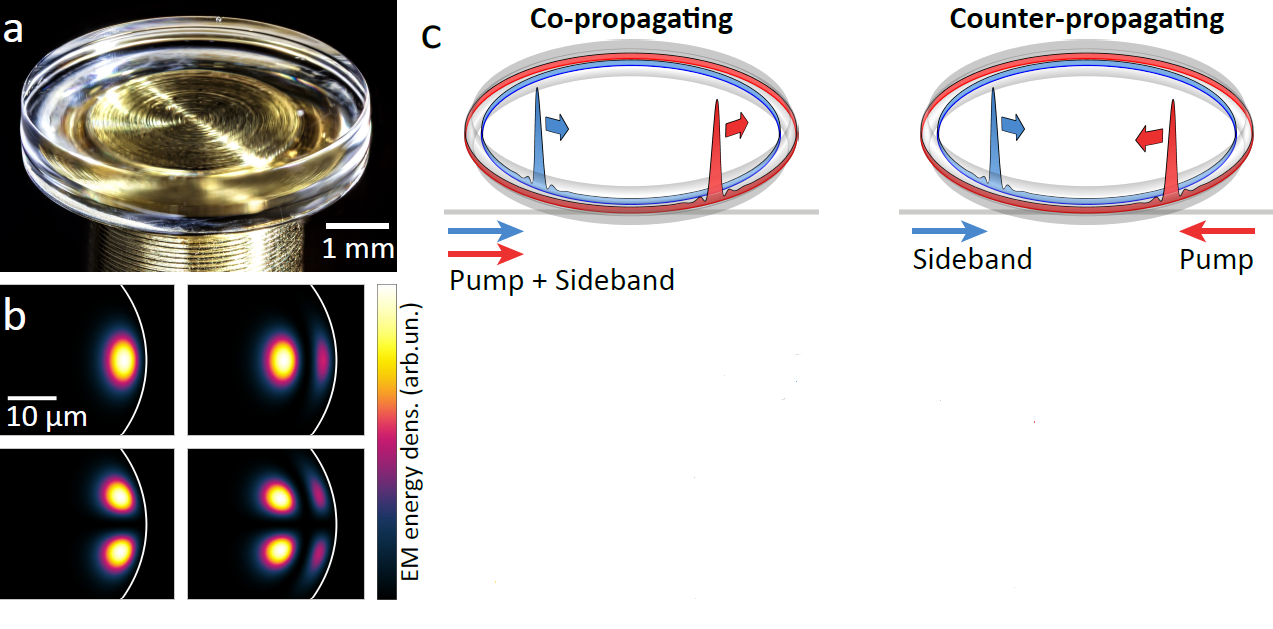
\includegraphics[width=0.75\linewidth]{fig1_scheme_general}}
\end{minipage}
\caption{(а) Фотография многомодового резонатора $MgF_2$, диаметр 5.5 мм; (b) примеры различных семейств мод и распределения электрического поля внутри МШГ; (с) схема возбуждения солитонов с распространением в одном или противоположных направлениях.}
\label{Figure1_V1_c}
\end{figure}

\begin{figure}[!htb]
\begin{minipage}{1\linewidth}
\center{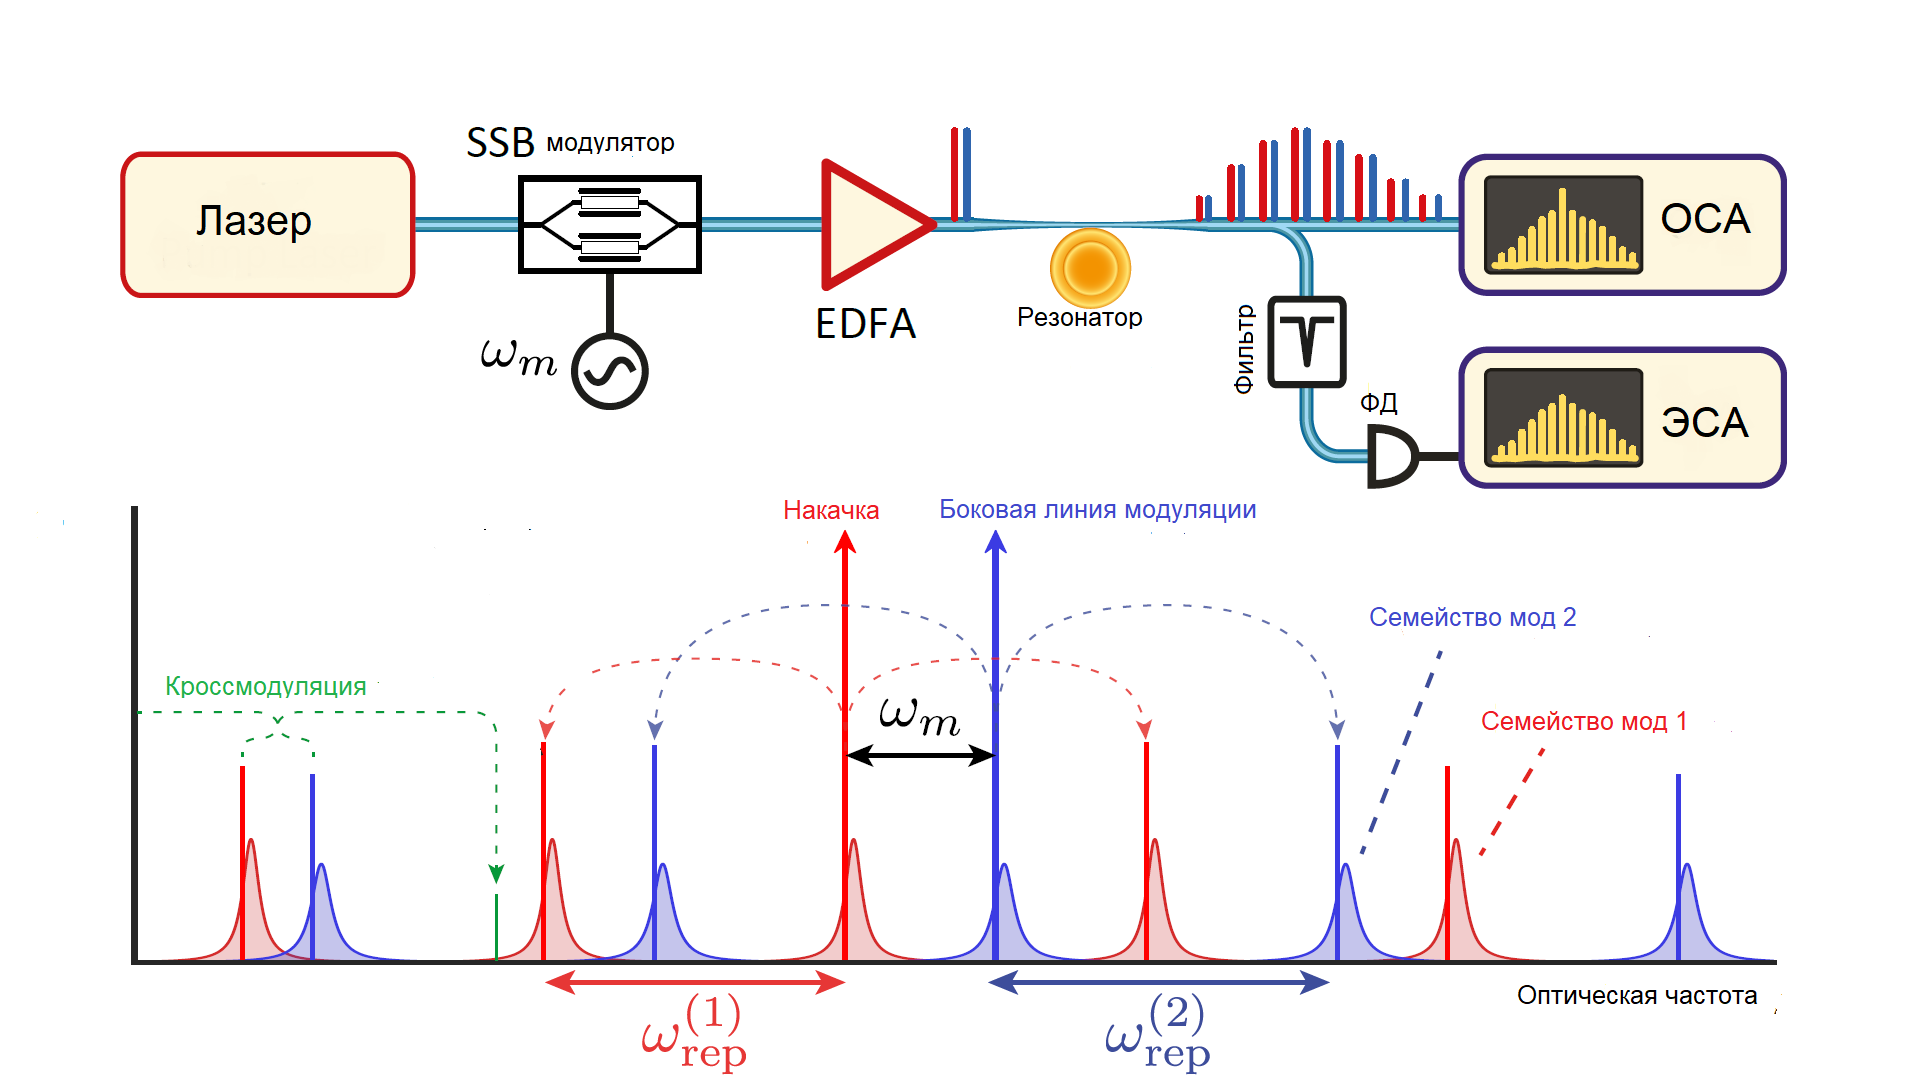
\includegraphics[width=0.75\linewidth]{fig1_scheme_setup}}
\end{minipage}
\caption{(Сверху) Схема экспериментальной установки: Лазер - волоконный перестраиваемый лазер непрерывной мощности, SSB модулятор - волоконный амплитудный модулятор с 1 боковой линией, EDFA - эрбиевый волоконный усилитель, резонатор, Фильтр - волоконный Брэгговский фильтр, ФД - быстрый фотодиод, ОСА - оптический спектроанализатор, ЭСА - анализатор спектра электрических сигналов. (снизу) концептуальная схема эксперимента, красным и синим изображены разные пространственные семейства мод в одном резонаторе, имеющие разные ОСД FSR1 и FSR2, расстояние между накачиваемыми двумя модами $f_m$ выбирается как частота модуляции, зеленым обозначен пример кроссмодуляции при взаимодействии солитонов}
\label{Figure1_V1_c}
\end{figure}


\begin{figure}[!htb]
\begin{minipage}{1\linewidth}
\center{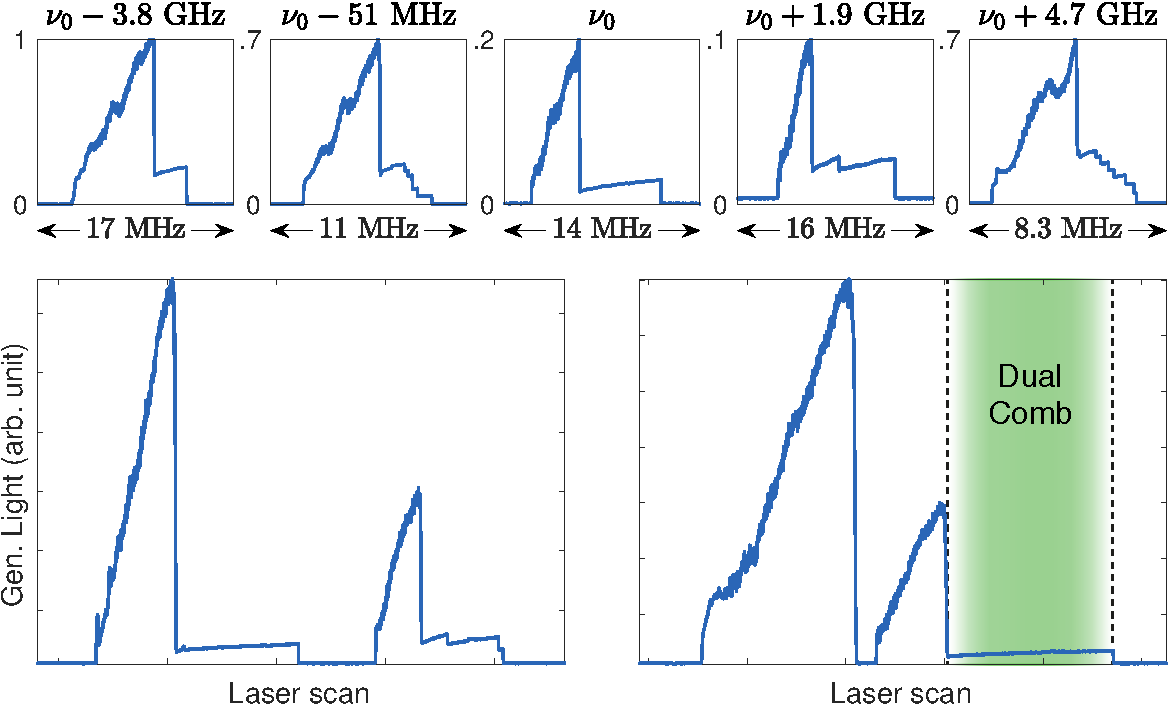
\includegraphics[width=0.5\linewidth]{Figure2}}
\end{minipage}
\caption{Сверху показаны сигналы генерируемого света для разных семейств мод, содержащие характерные солитонные ступеньки, даны отличия собственных частот для этих мод от выбранной центральной. Масштаб по вертикальной оси разный. Внизу показан метод совмещения солитонных ступенек при изменении частоты модуляции. Зеленой областью показан диапазон отстройки, при котором одновременно могут существовать солитоны на обоих семействах мод.}
\label{Figure2}
\end{figure}

%В ходе эксперимента удалось одновременно настроиться на оба солитона на разных семействах мод и стабилизировать отстройку частоты лазера, т.ч. солитоны существовали несколько часов. На рис. \ref{Co_Scheme_results} приведены экспериментальные результаты по одновременной генерации односолитонных режимов на двух разных семействах мод в одном резонаторе. Амплитуда лазера и 1 линии боковой модуляции были сделаны одинаковыми, частота модуляции составила 4.2817 ГГц, на этой же частоте наблюдалась результирующая гребенка в СВЧ диапазоне. Расстояние между линиями СВЧ гребенки составила 655 кГц, что равно разнице между частотами повторения солитонов на двух семействах мод. С помощью быстрого фотодетектора и осциллографа был измерена интерферограмма, которая подтвердила, что в результате мультигетеродинирования двух оптических солитонов образовался импульс в СВЧ диапазоне, огибающая которого соответствует огибающим в оптическом диапазоне. Также была измерена ширина одной нецентральной линии СВЧ гребенки, она составила 100 Гц (лимитирована разрешением прибора), что говорит об очень высокой взаимной когерентности оптических солитонов, которая в данном случае определяется стабильностью подаваемого СВЧ сигнала на модулятор и качеством стабилизации частоты отстройки лазера.

Итак, было продемонстрировано взаимно однозначное отображение оптического спектра солитонов (шириной 35 нм вокруг 1554 нм накачки) в СВЧ область (полной шириной около 200 МГц и центральной частотой около 4 ГГц).

\begin{figure}[!htb]
\begin{minipage}{1\linewidth}
\center{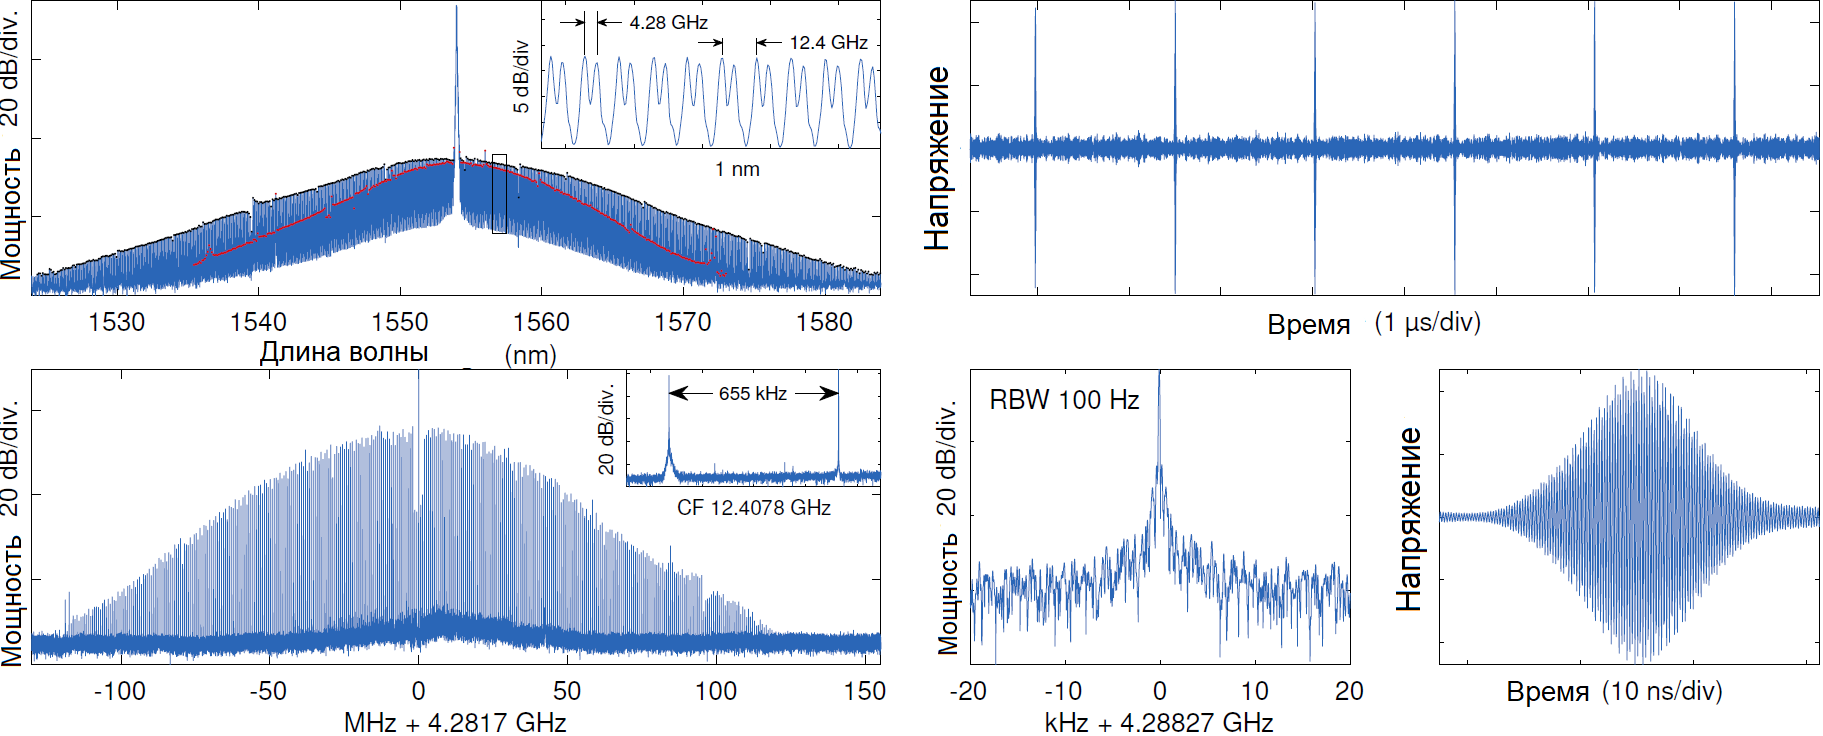
\includegraphics[width=1\linewidth]{Co_Scheme_results}}
\end{minipage}
\caption{Экспериментальные результаты одновременного возбуждения односолитонных режимов на двух разных семействах мод в 1 микрорезонаторе. (а) суммарный оптический спектр односолитонных режимов, красной линией помечена огибающая второго солитона, на вставке представлены отдельные линии двух солитонов. ОСД резонатора 12.4 ГГц, расстояние между несущими 4.28 ГГц. (б) результирующий сигнал биений двух солитонов - СВЧ гребенка с расстоянием между линиями 655 кГц, которое соответствует разнице между ОСД семейств мод, на вставке изображены сигналы частот повторения двух солитонов, (в) сигнал последовательности результирующих СВЧ импульсов, снятый быстрым осциллографом, (г) одиночная не центральная линия СВЧ гребенки шириной менее 100 Гц, (д) сигнал одиночного СВЧ импульса, соответствующий СВЧ гребенке.}
\label{Co_Scheme_results}
\end{figure}

\begin{figure}[!htb]
\begin{minipage}{1\linewidth}
\center{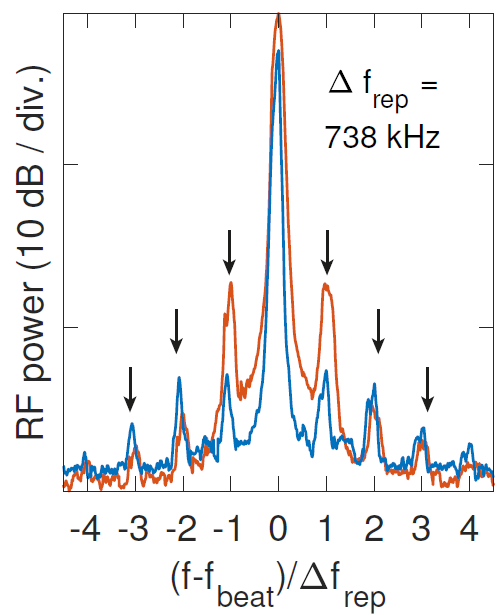
\includegraphics[width=0.3\linewidth]{fig4_intermodulation}}
\end{minipage}
\caption{Экспериментальное наблюдение слабых боковых линий у индивидуальной линии оптической гребенки, вызванных четырехволновым взаимодействием между линиями двух солитонных гребенок, распространяющихся в одном направлении на разных семействах мод. Частоты строго кратны разнице частот повторений солитонов, а максимальная мощность составляет -20 дБн}
\label{fig4_intermodulation}
\end{figure}

На рис. \ref{coscheme_different_types} приведены результаты генерации солитонов на другой паре семейств мод. Частота модуляции, равная разнице собственных частот мод из двух семейств, составила $4.9119$~ГГц, расстояние между ОСД семейств мод 9.2633~МГц, оно же являлось расстоянием между линиями СВЧ гребенки. В данном случае на одном семействе мод был достигнут односолитонный режим, а на другом многосолитонный. Хорошо видно совпадение огибающих оптического спектра солитонов и результирующего спектра СВЧ сигнала. Уровень компрессии составил $1.4\times10^3$, что ниже, чем для любых других продемонстрированных двойных гребенок из микрорезонаторов. Отметим видимый в этом эксперименте недостаток, при большом отличии ОСД между семействами мод, результирующая СВЧ гребенка перекрывается с собой, т.к. линии от мультигетеродинирования расположены вокруг центральных частот $f_m$ и $f_{rep}-f_m$. Этот же недостаток может проявляться и при достаточно малых $f_m$.

Измерение стабильности индивидуальной линии \ref{single_line_stability_cp} говорит о хорошей стабилизации частоты лазера накачки и температуры резонатора.

\begin{figure}[!htb]
\begin{minipage}{1\linewidth}
\center{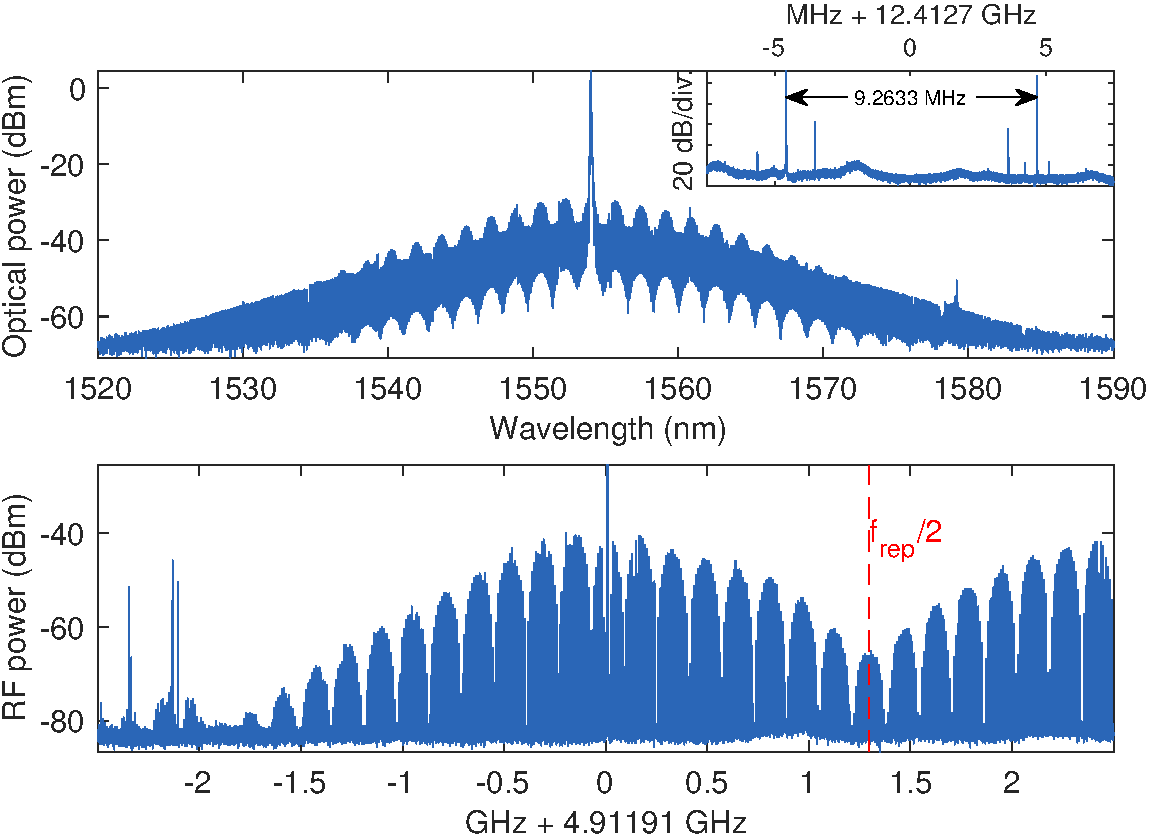
\includegraphics[width=0.75\linewidth]{coscheme_different_types}}
\end{minipage}
\caption{Результаты одновременной генерации солитонов в одном направлении на другой паре семейств мод. (сверху) суммарный оптический спектр односолитонного режима на одном семействе мод и многосолитонного режима на другом семействе мод, на вставке показана разница между частотами повторений 9.2633~МГц, (снизу) результирующая CВЧ гребенка с центральной частотой 4.9119 ГГц, видно что гребенка перекрывается с собой на половине частоты повторения солитонов (отмечено красной линией).}
\label{coscheme_different_types}
\end{figure}

\begin{figure}[!htb]
\begin{minipage}{1\linewidth}
\center{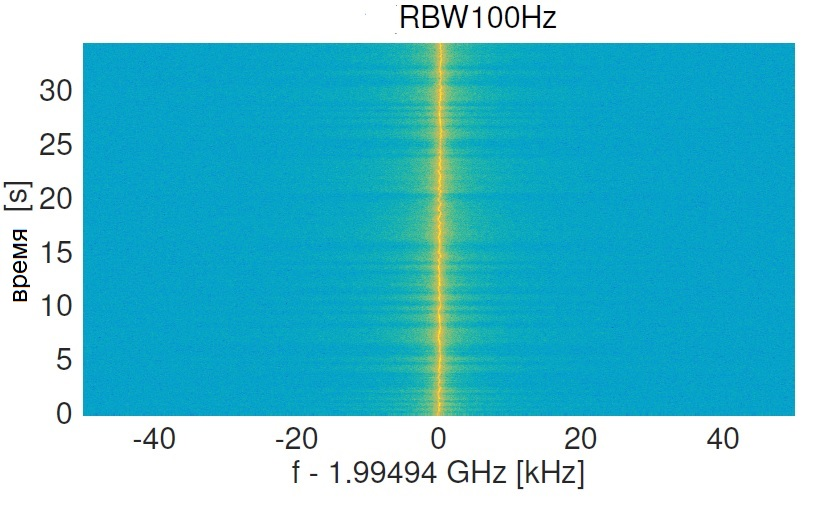
\includegraphics[width=0.5\linewidth]{single_line_stability_cp}}
\end{minipage}
\caption{Измерение стабильности индивидуальной линии СВЧ гребенки.}
\label{single_line_stability_cp}
\end{figure}

Отметим также технический недостаток схемы с двумя солитонами в одном направлении - сигнал ошибки схемы PDH несет информацию одновременно от обоих резонансов, что может мешать стабилизации, особенно при наличии эффекта пересечения мод хотя бы на одном солитонном резонансе.

Важным преимуществом схемы солитонов в одном направлении является ее относительная простота и отсутствие невзаимных устройств (изоляторов и циркуляторов). Практическим для некоторых приложений недостатком схемы с двумя солитонами в 1 направлении является невозможность разделить эти солитоны (у них одна поляризация и близкие оптические частоты), поэтому такая схема может не подойти, например, для фазово-чувствительной спектроскопии поглощения веществ и ЛИДАР применений.

\section{Генерация солитонных оптических гребенок в одном резонаторе на разных семействах мод в противоположных направлениях}

Чтобы разделить солитоны из одного резонатора был проведен следующий эксперимент с микрорезонатором из предыдущего пункта, в котором солитоны на разных семействах мод возбуждались в противоположных направлениях. Схема экспериментальной установки приведена на рис. \ref{Setup_CounterProp}. Волоконный перестраиваемый лазер непрерывной мощности усиливается эрбиевым усилителем, 0.1 мощности в одном плече после делителя модулируется амплитудным модулятором с одной боковой линией в таком режиме, что вся мощность перекачивается в эту боковую линию, далее сдвинутый по частоте лазерный сигнал усиливается и подается через оптический циркулятор в резонатор из $MgF_2$, другое плечо содержит 0.9 мощности исходного усиленного лазера (200 мВт) и подается через другой циркулятор на тот же элемент связи - растянутое волокно. Третьи выходы двух оптических циркуляторов в такой конфигурации содержат свет, прошедший через резонатор в противоположных направлениях. Брэгговские волоконные фильтры используются для подавления мощных несущих. Далее полученные сигналы независимо подаются на оптические спектроанализаторы и могут быть сбиты на волоконном делителе и отправлены на быстрый фотодетектор для генерации СВЧ гребенки.

Были использованы моды из пары семейств, с разницей в собственных частотах $f_m=2.75$ ГГц и разницей в частотах повторения $\Delta f_{rep}=371$ кГц для демонстрации пространственного мультиплексирования в противоположных направлениях. Настройка на солитонный режим производилась тем же методом, что и в случае распространения в одном направлении. Оптические спектры односолитонных режимов даны на рис. \ref{counter_prop_results}. Мощность каждого солитона после подавления накачки около 400 мкВт. Соответствующая СВЧ гребенка имела тот же уровень стабильности, что и в схеме с распространением в одном направлении, с шириной индивидуальной линии около 200 Гц. Основное преимущество схемы - это отсутствие кроссмодуляции между солитонами, т.к. для эффективного четырехволнового взаимодействия не выполняется условия сохранения углового момента для семейств мод в противоположных направлениях.

\begin{figure}[!htb]
\begin{minipage}{1\linewidth}
\center{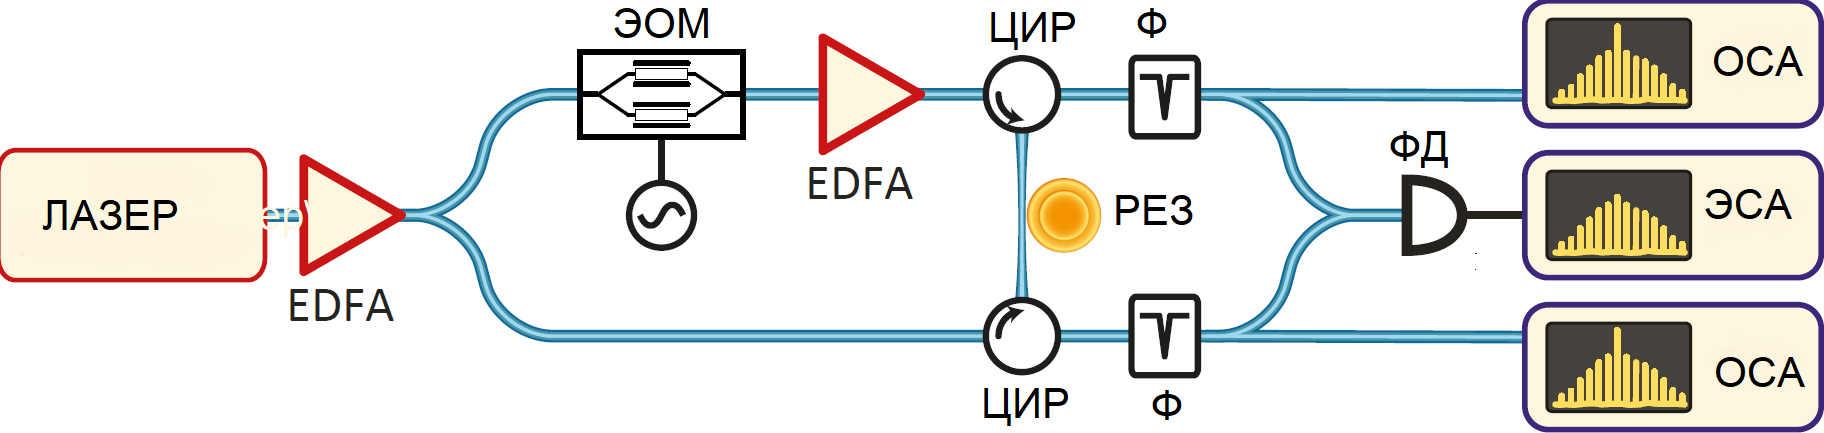
\includegraphics[width=0.75\linewidth]{Setup_CounterProp}}
\end{minipage}
\caption{Схема экспериментальной установки: Лазер - волоконный перестраиваемый лазер непрерывной мощности, ЭОМ - волоконный амплитудный модулятор с 1 боковой линией, EDFA - эрбиевый волоконный усилитель, Рез - микрорезонатор , Ф - волоконный Брэгговский фильтр, ФД - быстрый фотодиод, ОСА - оптический спектроанализатор, ЭСА - анализатор спектра электрических сигналов, ЦИР - оптический циркулятор}
\label{Setup_CounterProp}
\end{figure}

В эксперименте мощность накачек в обоих плечах выравнивалась, а частота модуляции подбиралась так, чтобы совпадали солитонные ступеньки в сигнале генерируемого света, также как и в случае солитонов в 1 направлении на разных семействах мод. Использовался метод PDH стабилизации частоты лазера к моде резонатора. Также была задействована схема активной стабилизации температуры резонатора. Экспериментальные результаты приведены на \ref{counter_prop_results}. Красный оптический спектр имеет сильно выраженный пик на 1530 нм, вероятно, связанный с сильным эффектом нормального расщепления мод. Результирующая картина СВЧ гребенки хорошо воспроизводит огибающие оптических спектров солитонов (однако присутствуют дополнительные компоненты на +70 МГц и -70 МГц, вероятно, связанные с техническими шумами). Результаты измерения девиации Аллана показывают, что разница частот повторений солитонов стабильнее, чем индивидуальная частота биений для 1 солитона, что говорит о хорошей работе системы привязки PDH. Для того чтобы минимизировать флуктуации амплитуд индивидуальных линий СВЧ гребенки необходимо бороться с паразитными переотражениями в схеме после резонатора, иначе образуются дополнительные резонаторы типа Фабри-Перо, и избегать флуктуаций фазы света в плечах, уменьшая длину волокон и контролируя их температуру и механические вибрации.

Продемонстрированный метод генерации двойной гребенки в противоположных направлениях на разных семействах мод подходит для проведения фазочувствительной спектроскопии. Был проведен демонстрирующий эту концепцию эксперимент: оба солитона были усилены до 10 мВт в эрбиевых волоконных усилителях, одна гребенка была пропущена через вейвшейпер (оптический генератор сигналов произвольной формы), потом сбита со второй гребенки на волоконном делителе. Амплитуда каждой линии в результирующей СВЧ гребенке сравнивалась с сигналом гребенки без пропускания через вейвшейпер. Использовался высокоскоростной осциллограф с временем сбора данных 1 мс, что соответствовало 370 усреднениям. Результаты измерения хорошо совпали с запрограммированным профилем, кроме краев спектра, где мощности линий гребенки крайне малы и ошибка в измерениях велика (см. рис. \ref{fig3_spectroscopy}).

\begin{figure}[!htb]
\begin{minipage}{1\linewidth}
\center{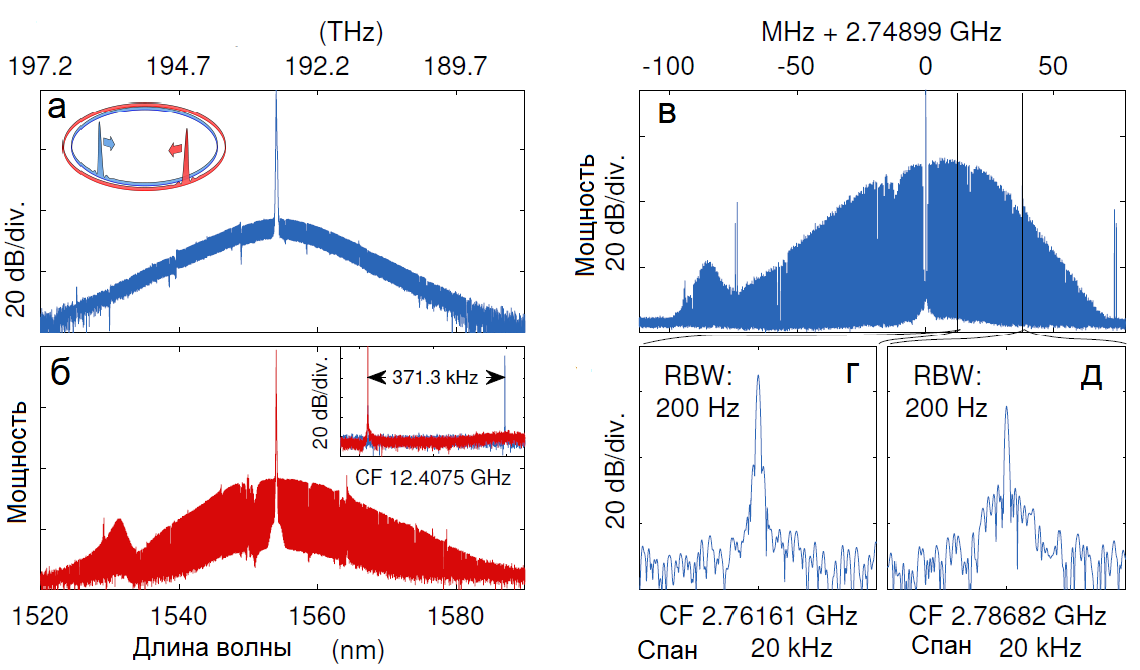
\includegraphics[width=1\linewidth]{counter_prop_results}}
\end{minipage}
\caption{Экспериментальные результаты одновременного возбуждения солитонов в противоположных направлениях в 1 резонаторе на разных семействах мод. (а,б) Оптические спектры односолитонных режимов, полученных на разных семействах. На вставке показаны наложенные друг на друга сигналы биений на частоте повторения солитонов. Разница в частотах повторений составила 371 кГц. (в) Результирующая СВЧ гребенка, получаемая на фотодетекторе при совмещении солитонов, распространяющихся в противоположном направлении, центральная частота совпадает с частотой модуляции 2.748 ГГц, расстояние между линиями 371 кГц. (г,д) Ширина индивидуальных линий СВЧ гребенки порядка 500 Гц.}
\label{counter_prop_results}
\end{figure}

\begin{figure}[!htb]
\begin{minipage}{1\linewidth}
\center{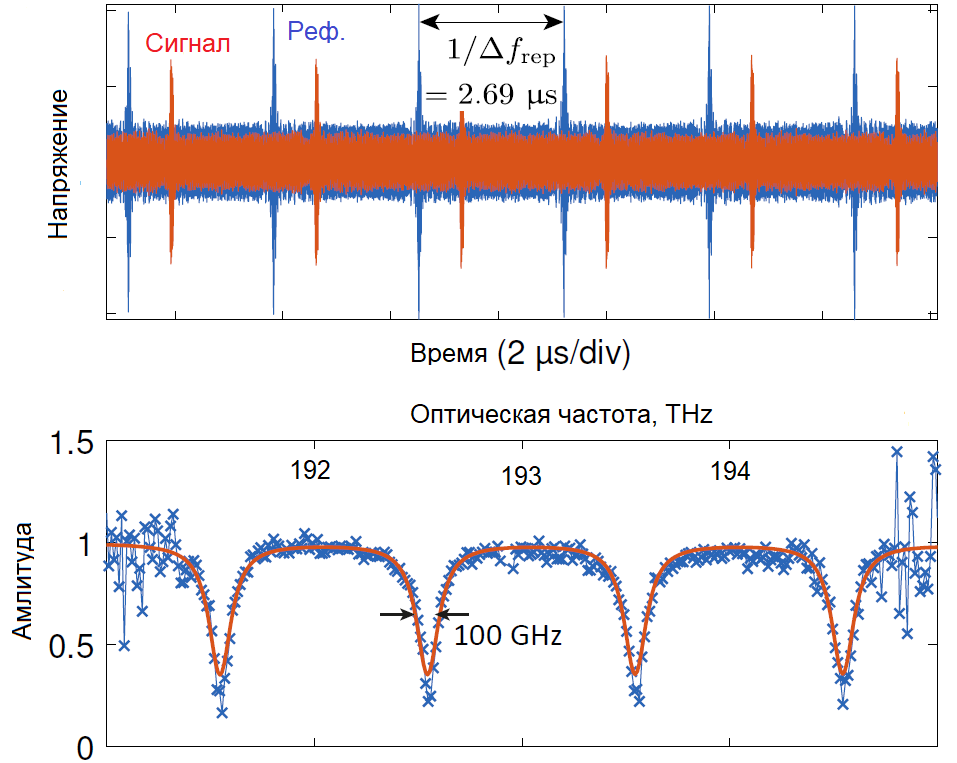
\includegraphics[width=0.7\linewidth]{fig3_spectroscopy}}
\end{minipage}
\caption{Экспериментальные результаты спектроскопии с использованием двойной гребенки. Сверху интерферограмма опорной гребенки и сигнальной, прошедшей через исследуемое вещество (сигнал вейвшейпера), снизу спектр пропускания: красным запрограммированный профиль пропускания вейвшейпера, синим измерение с помощью двойной гребенки.}
\label{fig3_spectroscopy}
\end{figure}


\section{Генерация солитонных оптических гребенок в одном резонаторе на одном семействе мод в противоположных направлениях}

Предложенный в предыдущем пункте метод генерации солитонов в 1 резонаторе в противоположных направлениях применим не только при накачке разных семейств мод, но возможен и на одном семействе мод. Используя схему (рис. \ref{Setup_CounterProp}) и экспериментальный метод из предыдущего пункта, возможно возбудить два солитона на 1 моде в противоположных направлениях (см. рис. \ref{cp_one_family}), для этого на амплитудный модулятор подается частота не выше максимальной отстройки, при которой существует солитон (типичные значения 5-20 МГц). Т.к. частота повторения солитонов зависит от отстройки частоты накачки от холодного резонанса, то при небольшом сдвиге накачки в прямом и обратном направлениях возможно образование результирующей СВЧ гребенки \ref{cp_one_family_dual_comb}. Важно отметить, что существует пороговое значение этой отстройки (частота на модуляторе менее 2 МГц), при которой частоты повторения солитонов строго совпадают и двойная гребенка не наблюдается. Также экспериментально обнаружено, что частоты повторений могут совпасть и при таком значении отстройки, когда возбуждаются сильные пересечения мод. Важно отметить, что использования одного лазера недостаточно, т.к. при нулевой отстройке накачек друг относительно друга по частоте, частоты повторений солитонов строго совпадают, даже если в одном направлении возбуждается многосолитонный режим с большей суммарной мощностью, а в противоположном направлении - односолитонный.

Измеренная стабильность индивидуальных линий (см. рис. \ref{cp_one_family_stability}) показывает сдвиг на 100 Гц за 60 сек, однако флуктуации амплитуды индивидуальных линий были высокими (Рис. \ref{cp_one_family_dual_comb} (b)), вероятной технически устранимой причиной являются сильные паразитные переотражения на коннекторах волокон волоконного делителя.

\begin{figure}[!htb]
\begin{minipage}{1\linewidth}
\center{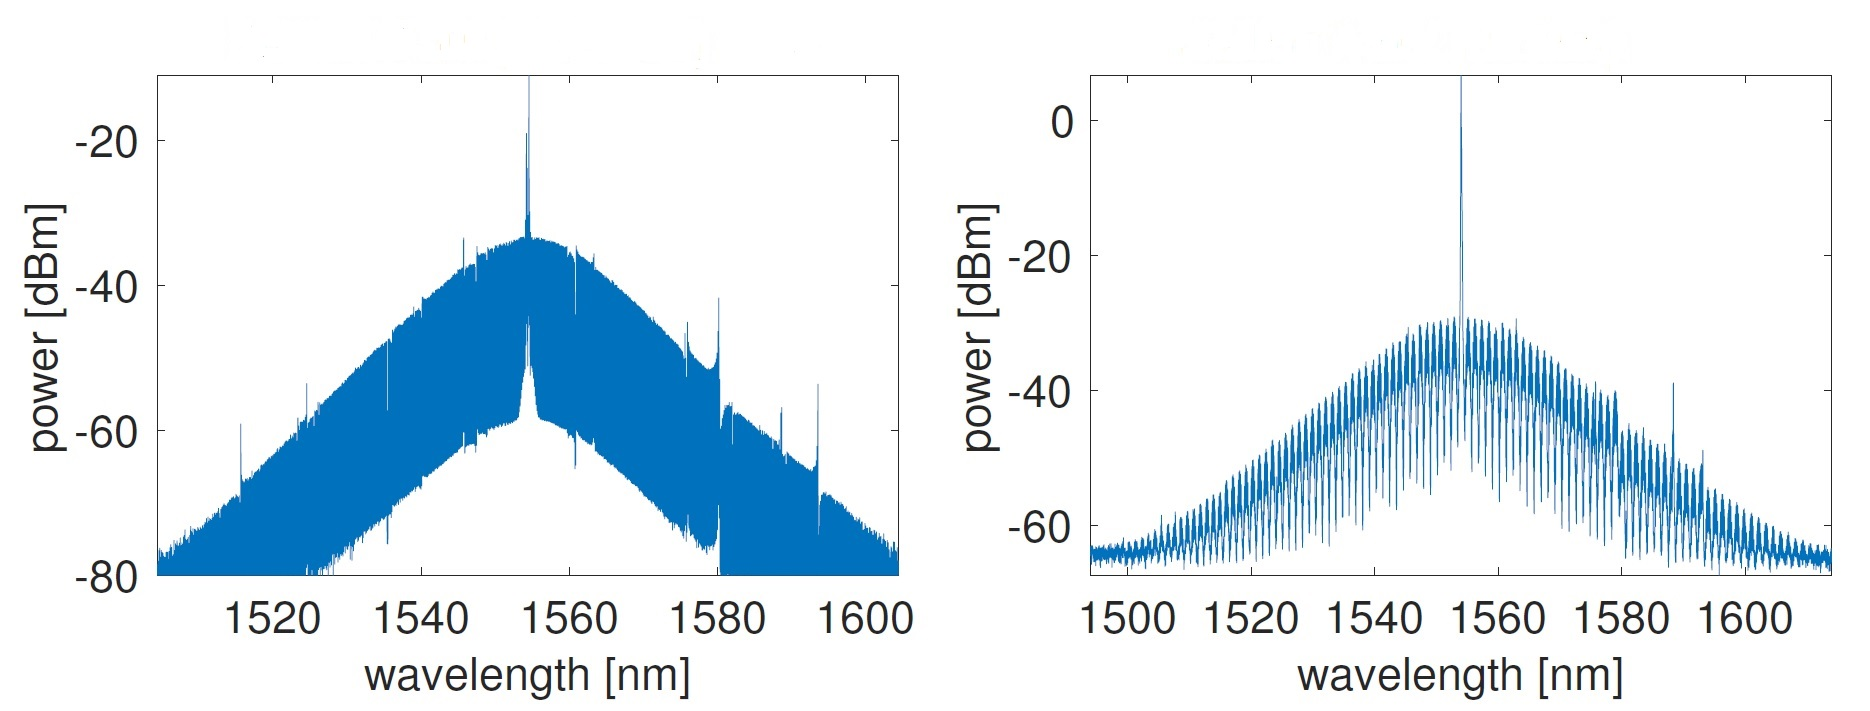
\includegraphics[width=0.7\linewidth]{cp_one_family}}
\end{minipage}
\caption{Экспериментальные результаты возбуждения солитонов в противоположных направлениях в 1 резонаторе на одном семействе мод. Оптические спектры: односолитонный режим в одном направлении, многосолитонный режим в противоположном направлении на том же семействе мод.}
\label{cp_one_family}
\end{figure}

\begin{figure}[!htb]
\begin{minipage}{1\linewidth}
\center{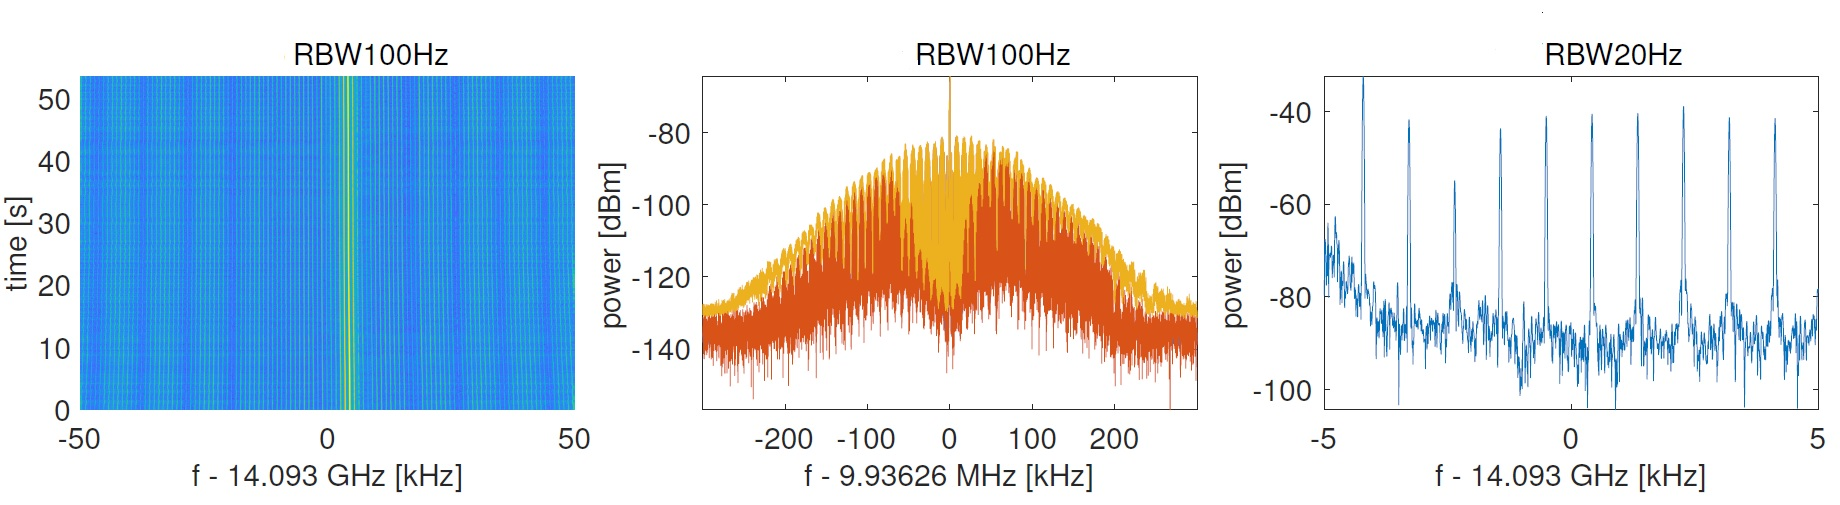
\includegraphics[width=1\linewidth]{cp_one_family_dual_comb}}
\end{minipage}
\caption{Результирующая СВЧ гребенка, получаемая на фотодетекторе при совмещении солитонов, распространяющихся в противоположном направлении на одном семействе мод, центральная частота совпадает с частотой модуляции 9.93 МГц, расстояние между линиями СВЧ гребенки порядка 1 кГц и растет с увеличением разности частот накачек. (слева) стабильность результирующей гребенки, (центр) спектр гребенки, желтым максимальное значение, красным - усредненное за 10 сек, (справа) спектр индивидуальных линий результирующей гребенки}
\label{cp_one_family_dual_comb}
\end{figure}

\begin{figure}[!htb]
\begin{minipage}{1\linewidth}
\center{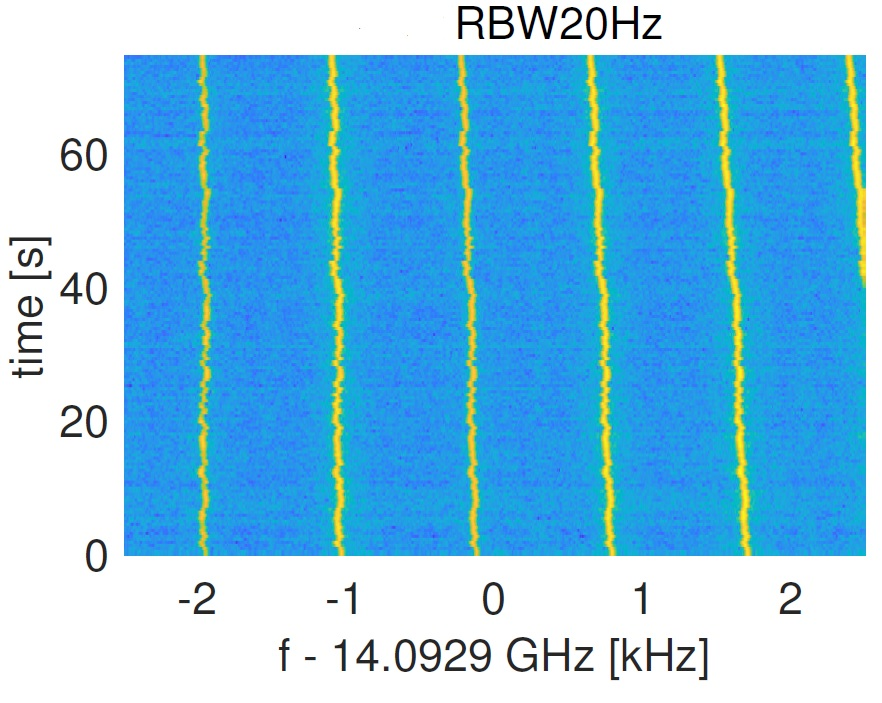
\includegraphics[width=0.5\linewidth]{cp_one_family_stability}}
\end{minipage}
\caption{Стабильность индивидуальных линий гребенки за 1 мин., полученной как биение двух солитонов, возбужденных на одном семействе мод в противоположных направлениях}
\label{cp_one_family_stability}
\end{figure}

Предложенный метод может быть удобен тем, что подходит для одномодовых резонаторов (например, интегральных) или резонаторов, не поддерживающих солитоны на разных семействах мод, а также тем, что не требует высоких частот, подаваемых на модулятор и быстрых фотодетекторов для регистрации двойных гребенок в СВЧ области.

\section{Выводы к главе 4}
Данная глава посвящена экспериментальному исследованию генерации двойных оптических частотных гребенок в микрорезонаторах. Продемонстрированы различные схемы одновременной генерации сразу двух солитонов: 1) в отдельных резонаторах на одном кристаллическом цилиндре при накачке двумя независимыми лазерами; 2) в одном резонаторе на разных пространственных семействах мод при накачке лазером и боковой линией амплитудного модулятора, солитоны распространялись как в одном, так и в противоположных направлениях; 3) в одном резонаторе на одном семействе мод при накачке лазером и боковой линией амплитудного модулятора, солитоны распространялись в противоположных направлениях. Проведено сравнение этих методов и описаны способы их улучшения. Экспериментально был продемонстрирован метод спектроскопии поглощения веществ с помощью двойной оптической частотной гребенки. Результаты главы 4 были опубликованы в статьях с номерами 7,9 из списка публикаций.


%Сошлемся на все конференции \cite{confbib1,confbib2,confbib3,confbib4,confbib5,confbib6,confbib7,confbib8,confbib9,confbib10,confbib11,confbib12,confbib13,confbib14}
%\section{Экспериментальное наблюдение вынужденного рассеяния Рамана и Бриллюэна в кристаллических микрорезонаторах} 